\section{Contexte}
\label{sec:contexte}

\subsection{Tracé de rayon et \textit{raymarching}}
\label{sec:ray-tracing-raymarching}

L'algorithme de tracé de rayon (\textit{ray tracing}) est l'algorithme utilisé pour effectuer le rendu des modèles dans ce projet. L'idée est plutôt simple : pour chaque pixel d'une caméra fictive, on lance un ou plusieurs rayons. Ces rayons trouvent de façon analytique leur intersection avec les modèles de la scène, rebondissent ensuite sur ces surfaces et accumulent la radiance des objets intersectés, ce qui représente la couleur du pixel correspondant.

L'algorithme de \textit{raymarching} fonctionne de façon similaire au tracé de rayon en lançant des rayons pour chaque pixel, mais plutôt que de trouver la prochaine intersection de façon analytique, il avance par pas discrets le long du rayon afin d'évaluer en chaque point si une collision se produit. Cet algorithme est particulièrement utile pour les volumes, lorsqu'on désire accumuler une valeur de densité ou de brouillard en traversant la scène. Une version spécialisée appelée \textit{sphere tracing} sera discutée dans la section~\ref{sec:sdf} consacrée aux fonctions de distance signée.

\subsection{Représentation d'une scène}
La représentation de scène en rendu fait référence à la manière dont les environnements 3D et leurs éléments constitutifs sont organisés et décrits pour être utilisés dans les pipelines de rendu. Ces représentations encodent différents types d'éléments, notamment des géométries d'objets, des personnages dotés de systèmes squelettiques et de cheveux, ainsi que des milieux participants comme la fumée, le brouillard ou la vapeur.

\subsubsection{Diversité des pipelines de rendu}

Différents types d'éléments de la scène nécessitent des approches de rendu spécialisées. Par exemple, Blender Cycles utilise un tracé de rayon volumétrique pour rendre les milieux participatifs, tout en employant le lancer de rayons standard pour les maillages d'objets. Cette séparation reflète les différences fondamentales entre l'interaction de la lumière avec les surfaces et avec les volumes.

Cette diversité de formats de représentation implique que les pipelines de rendu doivent prendre en charge plusieurs types d'éléments, chacun possédant des structures mémoire, des routines d'intersection et des modèles d'ombrage distincts.

Une approche unifiée capable de traiter surfaces et volumes avec une représentation unique pourrait simplifier considérablement les architectures de rendu. Cela constitue une partie de la motivation derrière l'exploration de techniques telles que les GPIS.

\subsection{Cheveux}

\subsubsection{État de l'art du rendu des cheveux}

Les cheveux et la fourrure sont omniprésents dans les médias rendus, des jeux vidéo aux personnages de films d'animation. Encore aujourd'hui, le rendu réaliste des fibres demeure un défi, tant en raison de leur complexité géométrique que de la diffusion lumineuse complexe d'une fibre à l'autre. La plupart des techniques modernes trouvent leur origine soit dans l'approche des \textit{hair cards} proposée par Kajiya et Kay \cite{kajiya1989rendering}, soit dans le paradigme de diffusion par fibres introduit par Marschner et al. \cite{marschner2003}.

Suite à la publication de Marschner, la recherche s'est concentrée sur la correction de certaines lacunes du modèle, notamment l'absence de conservation de l'énergie. C'est ce que \textcite{deon2011egsr} ont accompli, produisant aujourd'hui le modèle considéré comme le plus physiquement exact pour le nuançage des cheveux. Le modèle de \textcite{chiang2016} reprend celui de d'Eon en le reparamétrisant afin d'offrir des paramètres plus intuitifs pour les artistes, facilitant ainsi son intégration dans les moteurs de rendu. Aujourd'hui, le modèle de Chiang est utilisé par des moteurs de rendu tels que Houdini~\cite{Houdini} et Mitsuba~3~\cite{Mitsuba3}.

\paragraph{Modèle de Kajiya et Kay}

Le modèle de Kajiya et Kay (1989)~\cite{kajiya1989rendering} repose sur une représentation polygonale des cheveux, ce qui lui permet de s'intégrer facilement aux pipelines de rendu rasterisés. L'approche modélise les cheveux comme des fibres cylindriques et utilise un modèle de nuancage anisotrope prenant en compte la direction tangente du brin.

Cependant, le modèle de Kajiya et Kay présente des limites importantes : il traite les cheveux comme des cylindres opaques et ne tient pas compte de la transmission ni des réflexions internes. Or, le cheveu étant un matériau diélectrique et parfois translucide, cette omission conduit à un rendu moins réaliste, incapable de reproduire correctement les reflets colorés et les effets de rétroéclairage.

\paragraph{Modèle de Marschner}

Le modèle de Marschner (2003)~\cite{marschner2003} constitue une avancée majeure par rapport à Kajiya et Kay en proposant une modélisation plus réaliste des fibres. Le modèle considère les cheveux comme des cylindres diélectriques rugueux, permettant de simuler correctement la réflexion interne et la transmission.

Marschner identifie trois modes principaux d'interaction de la lumière avec un cheveu :

\begin{itemize}[noitemsep]
    \item \textbf{R (Reflection)} : la lumière se réfléchit sur la surface externe de la fibre, produisant le reflet blanc principal.
    \item \textbf{TT (Transmission-Transmission)} : la lumière pénètre dans la fibre, traverse son intérieur et ressort de l'autre côté, produisant une diffusion vers l'avant visible en contre-jour.
    \item \textbf{TRT (Transmission-Reflection-Transmission)} : la lumière pénètre dans la fibre, se réfléchit sur la surface interne opposée, puis ressort, générant le reflet secondaire coloré.
\end{itemize}

La fonction de diffusion peut s'écrire :

\begin{equation}
\begin{aligned}
S(\theta_i, \theta_r, \phi_i, \phi_r) &= \frac{M_R(\theta_h) N_R(\eta'(\eta, \theta_d), \phi)}{\cos^2(\theta_d)} \\
&+ \frac{M_{TT}(\theta_h) N_{TT}(\eta'(\eta, \theta_d), \phi)}{\cos^2(\theta_d)} \\
&+ \frac{M_{TRT}(\theta_h) N_{TRT}(\eta^*(\phi_h, \theta_d), \phi)}{\cos^2(\theta_d)}
\end{aligned}
\end{equation}

où $M$ représente la fonction de diffusion longitudinale (modélisée par des gaussiennes) et $N$ la fonction de diffusion azimutale. Le modèle utilise des coordonnées sphériques avec $\theta$ pour l'angle longitudinal et $\phi$ pour l'angle azimutal. Plusieurs angles dérivés sont employés :
\begin{itemize}
    \item L'angle de différence : $\theta_d = (\theta_r - \theta_i)/2$
    \item L'azimut relatif : $\phi = \phi_r - \phi_i$
    \item Les demi-angles : $\theta_h = (\theta_i + \theta_r)/2$ et $\phi_h = (\phi_i + \phi_r)/2$
\end{itemize}

En principe, ce schéma peut être prolongé pour des transmissions avec $n$ réflexions internes (TRRT, TRRRT, etc.), mais l'impact visuel des termes d'ordre supérieur au TRT est généralement négligeable.

\subsubsection{Comparaison des modèles de rendu des cheveux}

La figure \ref{fig:hair_comparison} illustre, à gauche, des cheveux rendus avec le modèle de Kajiya-Kay, au centre avec le modèle de Marschner, et à droite des cheveux réels sous des conditions d'éclairage similaires. On observe clairement que le modèle de Marschner permet une meilleure reproduction des reflets secondaires colorés et offre un aspect moins plat que le modèle de Kajiya-Kay, bien qu'il conserve une certaine uniformité et ne capture pas encore parfaitement la richesse visuelle des cheveux réels.

\begin{figure}[H]
    \centering
    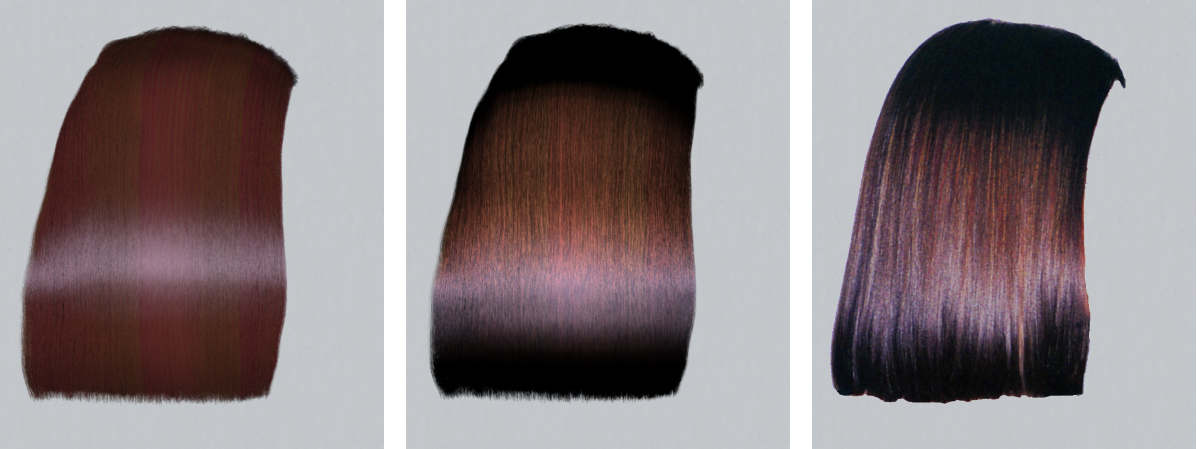
\includegraphics[width=\textwidth]{img/hair_comparison.png}
    \caption{Comparaison des modèles de rendu des cheveux : Kajiya-Kay (gauche), Marschner (centre) et cheveux réels (droite) sous un éclairage similaire. Image tirée de \textcite{marschner2003}.}
    \label{fig:hair_comparison}
\end{figure}

\paragraph{Modèle de d'Eon et al.}
Depuis la publication du modèle de Marschner, plusieurs travaux ont cherché à l'améliorer. Le plus important est celui de \textcite{deon2011egsr}, qui introduit la conservation de l'énergie. En effet, le modèle de Marschner ne garantit pas que la quantité totale de lumière diffusée soit inférieure ou égale à la quantité incidente : dans certaines configurations d'éclairage, il peut émettre plus de lumière qu'il n'en reçoit, ce qui produit des artefacts de sur-luminosité dans les scènes à forte densité de fibres. D'Eon et al. conservent la même décomposition factorisée que Marschner :
\begin{equation}
    S(\theta_i, \theta_r, \phi) = \sum_{p=0}^{\infty} M_p(\theta_i, \theta_r)\, N_p(\theta_i, \theta_r, \phi)
\end{equation}
mais reformulent les fonctions $M_p$ et $N_p$ pour garantir la conservation de l'énergie. La fonction longitudinale $M_p$, auparavant modélisée par une gaussienne, est remplacée par une convolution gaussienne sphérique qui corrige les pertes d'énergie aux angles rasants et à forte rugosité. La fonction azimutale $N_p$ est quant à elle obtenue par intégration numérique sur l'ensemble de la fibre via une quadrature de Gauss, évitant ainsi la résolution d'équations cubiques et traitant les caustiques de manière cohérente. Cette formulation s'étend naturellement aux ordres supérieurs (TRRT, TRRRT\ldots), contrairement au modèle de Marschner qui se limitait aux trois premiers modes R, TT et TRT. 
Ce modèle, formalisé sous la forme d'une \textit{Bidirectional Curve Scattering Distribution Function} (BCSDF), est désormais la référence dans les moteurs de rendu de l'industrie, et c'est cette représentation que nous utiliserons dans notre implémentation.

\subsubsection{Géométrie des cheveux}
\label{sec:geometrie-cheveux}

Bien qu'il soit possible de représenter la chevelure comme un maillage de triangles, les moteurs de rendu photoréalistes préfèrent une approche qui modélise chaque cheveu individuellement. Dans \textit{Physically Based Rendering}~\autocite{pbrt4}, les cheveux sont représentés par des courbes de Bézier cubiques, définies par quatre points de contrôle $p_0, p_1, p_2, p_3$. La courbe passe par le premier et le dernier point de contrôle, et les points intermédiaires sont déterminés par le polynôme :

\begin{equation}
    p(u) = (1-u)^3\,p_0 + 3(1-u)^2 u\,p_1 + 3(1-u)\,u^2\,p_2 + u^3\,p_3, \quad u \in [0,1]
\end{equation}

À chaque point de la courbe, une largeur est interpolée linéairement entre une valeur initiale et une valeur finale, définissant ainsi une surface plate orientée vers la caméra. Cette représentation permet d'intercepter les rayons directement sur la courbe sans la discrétiser en triangles, ce qui réduit considérablement la mémoire nécessaire tout en conservant un profil lisse. C'est cette primitive géométrique que nous utiliserons pour représenter les fibres de cheveux dans notre implémentation.

\paragraph{Format de fichier}

Un avantage pratique de cette représentation par courbes est la disponibilité de formats d'encodage standardisés. Mitsuba~3 utilise un format texte simple où chaque point de contrôle est encodé sur une ligne par un vecteur à quatre composantes $(x, y, z, r)$, où $x, y, z$ désignent la position dans l'espace et $r$ le rayon de la fibre en ce point. Les courbes sont séparées par une ligne vide, et chaque courbe nécessite au minimum quatre points de contrôle. Par exemple, le fichier suivant définit trois segments de courbe B-spline cubique :

\begin{verbatim}
2.43218 14.4892 -2.50452 0.002833
2.57673 14.5219 -2.57965 0.002833
2.69117 14.4482 -2.67604 0.002833
2.78262 14.3006 -2.78176 0.002833

2.57673 14.5219 -2.57965 0.002717
2.69117 14.4482 -2.67604 0.002717
2.78262 14.3006 -2.78176 0.002717
2.85818 14.1115 -2.88489 0.002717

2.69117 14.4482 -2.67604 0.0026015
2.78262 14.3006 -2.78176 0.0026015
2.85818 14.1115 -2.88489 0.0026015
2.92495 13.9132 -2.97351 0.0026015
\end{verbatim}

On notera que le rayon varie légèrement d'un segment à l'autre, permettant de modéliser l'effilement naturel du cheveu vers sa pointe. Ce format sera celui utilisé pour charger la géométrie capillaire dans notre pipeline de rendu.

\begin{figure}[H]
    \centering
    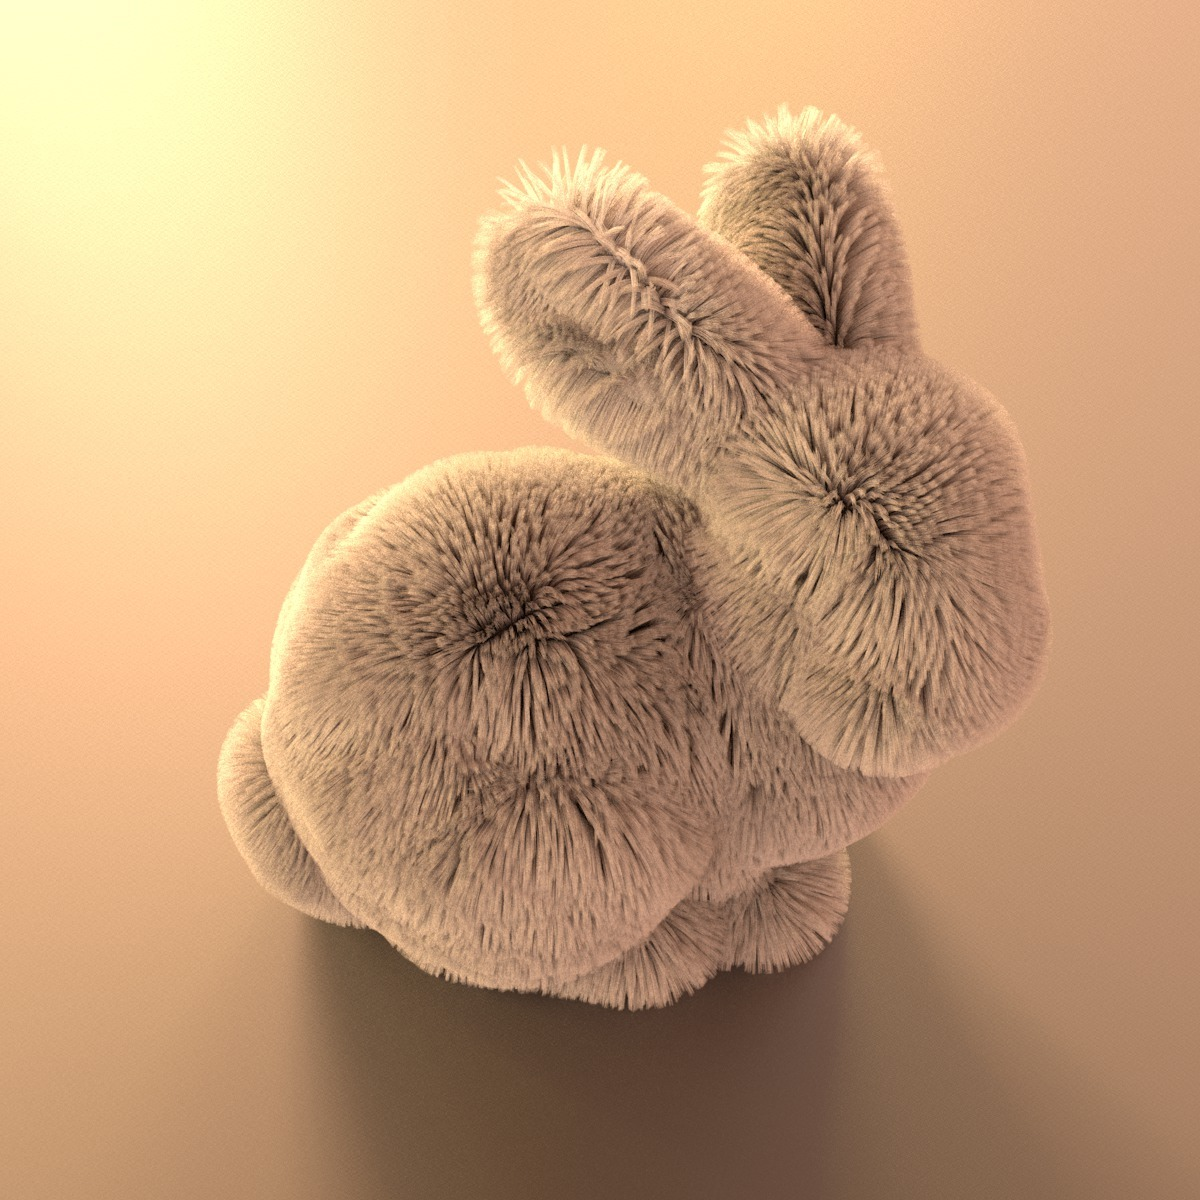
\includegraphics[width=0.6\textwidth]{figures/bunny-hair.jpg}
    \caption{Exemple tiré de \textcite{pbrt4} : le lapin de Stanford recouvert de courbes de Bézier cubiques pour représenter la fourrure.}
    \label{fig:bunny-hair}
\end{figure}

\subsection{Processus gaussiens}

Les processus gaussiens (GP) constituent un cadre d'apprentissage automatique qui considère l'ensemble des fonctions possibles pouvant approximer un jeu de données, en assignant une probabilité à chacune d'elles \cite{rasmussen2006gaussian}. L'hypothèse clé est que des points d'entrée similaires doivent produire des sorties similaires, ce qui permet au modèle de fournir à la fois une estimation ponctuelle et un degré d'incertitude pour chaque prédiction.

Les processus gaussiens sont définis par deux fonctions :

\begin{enumerate}[noitemsep]
    \item \textbf{La fonction moyenne $\mu(\mathbf{x})$}, qui représente les croyances a priori sur la fonction sous-jacente
    \item \textbf{Le noyau de covariance $k(\mathbf{x}, \mathbf{x}')$}, qui représente la corrélation entre deux points
\end{enumerate}

Les processus gaussiens fournissent une moyenne postérieure représentant la valeur prédite ainsi qu'une variance exprimant l'incertitude associée.

\subsubsection{Noyaux}
\label{sec:noyaux}
La fonction noyau est utilisée pour définir la matrice de covariance en encodant la corrélation entre deux points.

Le choix du noyau a un impact important sur la fonction sous-jacente inférée par le modèle ; le noyau choisi définit une hypothèse sur la régularité et la périodicité de celle-ci \cite{martens2016gpis}.

\paragraph{Noyau exponentiel quadratique (RBF)}

Le noyau exponentiel quadratique (RBF) est défini par :

\begin{equation}
k_{SE}(\mathbf{x}, \mathbf{x}') = \sigma^2 \exp \left(- \frac{1}{2\ell^2} \|\mathbf{x} - \mathbf{x}'\|^2 \right)
\end{equation} 
\cite{martens2016gpis}

où $\sigma^2$ est la variance du signal et $\ell$ le paramètre d'échelle.

Ce noyau est celui retenu pour ce projet, car il assure une interpolation lisse entre les points connus ; de plus, il est infiniment différentiable, ce qui est une propriété importante pour le rendu avec les GPIS. Le paramètre d'échelle $\ell$ contrôle la rapidité du changement du modèle entre les points.

\subsubsection{Conditionnement}
Le conditionnement d'un processus gaussien consiste à incorporer des données observées afin d'affiner les prédictions. Les équations de conditionnement et d'échantillonnage sont dérivées dans \textcite{martens2016gpis} et \textcite{seyb24from}; nous adoptons la notation de \textcite{seyb24from} qui est plus explicite. Étant donné des mesures $\mathbf{m}$ aux positions $\mathbf{C}$, le processus gaussien conditionné s'écrit :
\begin{equation}
f \sim \text{GP}\left(\mu_{|\zeta_m}(\mathbf{x}), k_{|\zeta_m}(\mathbf{x}, \mathbf{x}')\right)
\end{equation}

avec :
\begin{align}
\mu_{|\zeta_m}(\mathbf{x}) &= \mu(\mathbf{x}) + k(\mathbf{x}, \mathbf{C}) k(\mathbf{C}, \mathbf{C})^{-1} (\mathbf{m} - \mu(\mathbf{C})) \\
 k_{|\zeta_m}(\mathbf{x}, \mathbf{x}') &= k(\mathbf{x}, \mathbf{x}') - k(\mathbf{x}, \mathbf{C}) k(\mathbf{C}, \mathbf{C})^{-1} k(\mathbf{C}, \mathbf{x}')
\end{align}

\subsubsection{Échantillonnage}

L'échantillonnage d'un processus gaussien peut être réalisé via :

\begin{equation}
\label{eq:echantillonnage}
f(\mathbf{X}) = \mu(\mathbf{X}) + k(\mathbf{X}, \mathbf{X})^{1/2} \boldsymbol{\eta}
\end{equation}

où :
\begin{itemize}[noitemsep]
    \item $\boldsymbol{\eta} \sim \mathcal{N}(\mathbf{0}, \mathbf{I})$
    \item $\mathbf{A}^{1/2}$ est la racine carrée matricielle telle que $\mathbf{A} = \mathbf{A}^{1/2}\mathbf{A}^{1/2}$
\end{itemize}

\subsection{Surfaces implicites et fonctions de distance signée}
\label{sec:sdf}

Une surface implicite est définie par une fonction $f(\mathbf{x})$, où la surface correspond à l'ensemble des points tels que $f = 0$. Par convention, les points où $f > 0$ sont considérés comme étant à l'intérieur d'un objet et ceux où $f < 0$ à l'extérieur, bien que cette convention puisse être inversée. Les plus connues d'entre elles sont les fonctions de distance signée.

\subsubsection{Fonction de distance signée}

Les fonctions de distance signée (SDF) sont bien étudiées, car elles permettent de faire du rendu procédural avec l'algorithme \textit{raymarching}. L'idée est plutôt simple : on cherche à définir une forme par l'expression de la distance au point le plus proche sur la surface à partir d'un point sur le rayon.

L'exemple trivial est celui d'une sphère, dont la surface est obtenue avec la formule :
\begin{equation}
d = |\mathbf{p} - \mathbf{c}| - r
\end{equation}
soit la distance entre le centre $\mathbf{c}$ et le point sur le rayon $\mathbf{p}$, moins le rayon de la sphère $r$. Une multitude de fonctions ont été présentées par Iñigo Quílez pour des formes 2D et 3D \cite{quilez_sdf}.

Les SDF peuvent être utilisées comme surfaces implicites lorsque la distance signée est égale à zéro, ce qui indique que le point se trouve sur la surface de l'objet.

\paragraph{Sphere tracing}

Une propriété intéressante des SDF est que traverser une scène constituée d'objets SDF peut être réalisé efficacement avec le \textit{sphere tracing}. Cet algorithme est une optimisation du \textit{raymarching}, mais avec des pas dictés par la distance obtenue avec les SDF plutôt qu'avec des pas constants. Puisque chaque SDF peut être évaluée en $O(1)$, on évalue toutes les distances en $O(n)$ pour $n$ objets dans la scène.

\begin{figure}[H]
    \centering
    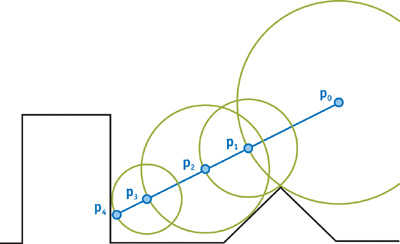
\includegraphics[width=0.7\textwidth]{figures/sphere_tracing.jpg}
    \caption{Visualisation de l'algorithme \textit{sphere tracing} : chaque pas le long du rayon est borné par la distance à la surface la plus proche.}
    \label{fig:sphere-tracing}
\end{figure}

\paragraph{SDF de la capsule}

La SDF importante pour ce projet est celle de la capsule. Une capsule est un segment de droite avec un rayon, analogue à un cylindre à extrémités hémisphériques. Elle est définie par deux points $\mathbf{a}$ et $\mathbf{b}$ et un rayon $r$ :

\begin{lstlisting}[language=C, caption={SDF d'une capsule, tirée de \cite{quilez_sdf}.}]
float sdCapsule(vec3 p, vec3 a, vec3 b, float r) {
    vec3 pa = p - a;
    vec3 ba = b - a;
    float h = clamp(dot(pa, ba) / dot(ba, ba), 0.0, 1.0);
    return length(pa - ba * h) - r;
}
\end{lstlisting}

En projetant le vecteur $\mathbf{pa} = \mathbf{p} - \mathbf{a}$ sur le vecteur $\mathbf{ba} = \mathbf{b} - \mathbf{a}$, on obtient le paramètre $h \in [0, 1]$ représentant la position du point le plus proche sur le segment. La distance entre ce point et $\mathbf{p}$, diminuée du rayon, correspond à la distance signée vers la capsule. Cet algorithme est identique en 2D et en 3D.

\begin{figure}[H]
    \centering
    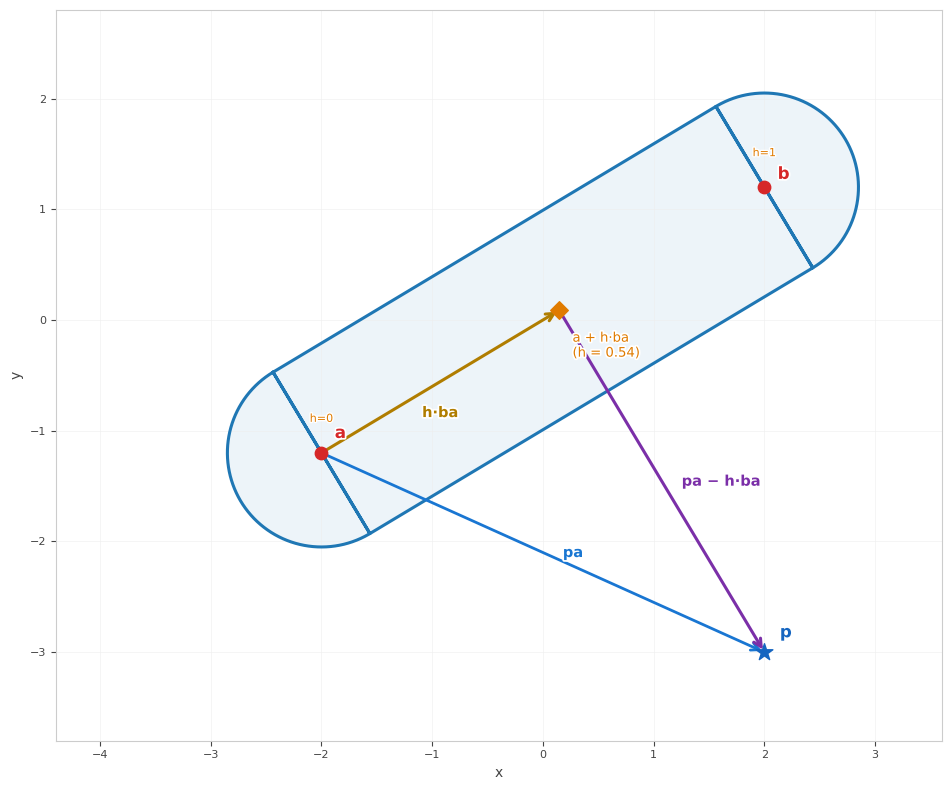
\includegraphics[width=0.7\textwidth]{figures/capsule-sdf.png}
    \caption{Démonstration visuelle de la fonction de distance signée de la capsule.}
    \label{fig:capsule_sdf}
\end{figure}

Un autre type de surface implicite est la surface implicite définie par processus gaussien.

\subsection{Surfaces implicites par processus gaussiens}

Les surfaces implicites définies par processus gaussiens (GPIS) ont été introduites par \textcite{williams2007gaussian} comme une approche probabiliste de reconstruction de surface~\cite{martens2016gpis}.

Les données d'entraînement d'un GPIS comprennent :

\begin{itemize}[noitemsep]
    \item Un ensemble de points sur la surface (où $f = 0$)
    \item Un ensemble de points connus à l'intérieur de la surface (où $f > 0$)
    \item Un ensemble de points connus à l'extérieur de la surface (où $f < 0$)
\end{itemize}

Si des normales associées aux points sont disponibles, on peut générer automatiquement des points intérieur/extérieur en décalant légèrement le long et contre la normale.

Le processus gaussien apprend une fonction qui interpole de manière lisse toutes les observations. La moyenne du processus gaussien représente la fonction implicite la plus probable, tandis que la variance fournit des estimations d'incertitude. La surface implicite correspond à l'ensemble des points où $f(\mathbf{x}) = 0$.

\subsubsection{Représentation d'élément par processus gaussiens}

Les GPIS sont particulièrement intéressants pour représenter des formes numérisées à partir de données LiDAR ou de caméras RGB-D. À partir d'un nuage de points, il est possible de conditionner le processus gaussien en définissant les points du nuage comme observations (avec $f = 0$). Cela crée une surface qui peut être rendue à l'aide d'algorithmes de \textit{raymarching} par recherche de racines, afin de déterminer l'intersection avec la surface définie par $f(\mathbf{x}) = 0$.

Pour les modèles basés sur des triangles, il est possible de conditionner le processus gaussien en :

\begin{enumerate}[noitemsep]
    \item Ajoutant chaque sommet du maillage comme observation de surface ($f = 0$)
    \item Exploitant les normales aux sommets pour inclure des points à l'extérieur du modèle ($f = -1$) et à l'intérieur ($f = +1$) en décalant dans la direction de la normale
\end{enumerate}

Pour les nuages de points issus de scans LiDAR, les normales ainsi que les points intérieurs et extérieurs doivent être déduits de la géométrie locale. Cela peut être réalisé en estimant les normales de surface à partir du gradient du processus gaussien. \cite{martens2016gpis}

Le processus gaussien conditionné définit une surface implicite qui interpole de manière lisse les données observées tout en fournissant des estimations d'incertitude loin des observations. La surface reconstruite est visible à la figure~\ref{fig:gpis_surfaces}.

\begin{figure}[H]
    \centering
    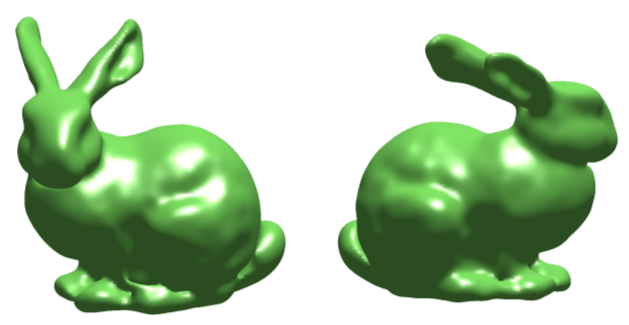
\includegraphics[width=0.5\textwidth]{img/gpis.png}
    \caption{Le Stanford bunny défini par 800 points de surface, un point intérieur $+1$, et une sphère de 80 points extérieurs $-1$ générés par l'algorithme marching cubes. Image tirée de \textcite{williams2007gaussian}.}
    \label{fig:gpis_surfaces}
\end{figure}

\subsubsection{Dérivées des processus gaussiens et normales de surface}

Une propriété fondamentale des processus gaussiens est que les dérivées d'un processus gaussien sont également des processus gaussiens. Cette propriété est essentielle pour les GPIS, car les normales de surface sont dérivées du gradient de la fonction implicite.

\paragraph{Processus gaussiens dérivés}

En raison de la linéarité de l'opérateur de dérivation, la dérivée d'un processus gaussien prend la forme :

\begin{equation}
\text{GP}'(\mu(\mathbf{x}), k(\mathbf{x}, \mathbf{x}')) = \text{GP}\left(\mu'(\mathbf{x}), k_{xx'}(\mathbf{x}, \mathbf{x}')\right)
\end{equation}

où :

\begin{equation}
k_{xx'}(\mathbf{x}, \mathbf{x}') = \frac{\partial^2 k(\mathbf{x}, \mathbf{x}')}{\partial \mathbf{x} \partial \mathbf{x}'}
\end{equation}

\paragraph{Calcul des normales sur les GPIS}

Pour une surface implicite définie par $f(\mathbf{x}) = 0$, la normale de surface en tout point est donnée par le gradient normalisé :

\begin{equation}
\mathbf{n}(\mathbf{x}) = \frac{\nabla f(\mathbf{x})}{||\nabla f(\mathbf{x})||}
\end{equation}


\subsubsection{Approximation d'un processus gaussien par convolution de bruit blanc}

Dans la fonction d'échantillonnage (équation~\ref{eq:echantillonnage}), on remarque que l'opération nécessite d'inverser la matrice de covariance $k(\mathbf{X}, \mathbf{X})$, dont le coût est en $O(n^3)$ pour $n$ points. C'est pourquoi \textcite{xu25practical} se sont intéressés à une technique d'approximation du processus gaussien par convolution parcimonieuse de bruit blanc permettant l'échantillonnage en temps constant. 

\paragraph{Le bruit blanc gaussien comme processus gaussien}

Le point de départ est le bruit blanc gaussien $W$, que l'on définit formellement comme un processus stochastique gaussien de moyenne nulle et dont la structure de covariance est entièrement caractérisée par un facteur de Dirac ($\delta$) :

\begin{equation}
\mathbb{E}[W(\mathbf{s})] = 0, \qquad \mathbb{E}[W(\mathbf{s})\, W(\mathbf{u})] = \sigma^2\, \delta(\mathbf{s} - \mathbf{u})
\end{equation}

Le terme $\delta(\mathbf{s} - \mathbf{u})$ exprime que deux évaluations du processus en des points distincts sont strictement décorrélées : toute la variance est concentrée de façon infiniment localisée sur la diagonale. $W$ est donc un $\text{GP}(0,\, \sigma^2 \delta)$.

\paragraph{Construction d'un processus gaussien lisse par convolution}

La convolution de $W$ avec un noyau $h$ produit un processus gaussien $\psi_{\text{dense}} \sim \text{GP}(0, k_{\text{dense}})$ dont la covariance s'écrit :

\begin{equation}
k_{\text{dense}}(\mathbf{x},\mathbf{x}') = \sigma^2 \int h(\mathbf{s}, \mathbf{x})\; h(\mathbf{s}, \mathbf{x}')\; d\mathbf{s}
\end{equation}

En choisissant un noyau de convolution gaussien stationnaire, cette intégrale se résout analytiquement et l'on retrouve la forme canonique du noyau RBF en dimension 3 :

\begin{equation}
k(\mathbf{r}) = \frac{\sigma^2}{8\pi^{3/2}\ell^{3}}\; \exp\!\left(-\frac{|\mathbf{r}|^2}{4\ell^2}\right)
\end{equation}

La dérivation complète de ce résultat est présentée à l'annexe~\ref{ann:derivation-se}.

Bien que nous ayons défini théoriquement le processus $\psi_{\text{dense}}$, l'évaluation via l'intégrale n'est pas utilisable en pratique ; il est toutefois possible de l'approximer par un bruit impulsionnel.

\paragraph{Approximation par convolution de bruit impulsionnel}

\paragraph{Motivation}

\textcite{lewis1986methods,lewis1989algorithms} ont proposé d'approcher le bruit blanc continu $W(\mathbf{s})$ par un processus d'impulsions aléatoires (processus de Poisson) :

\begin{equation}
W(\mathbf{s}) \approx W_\lambda(\mathbf{s}) := \sum_i w_i\, \delta(\mathbf{s} - \mathbf{s}_i)
\end{equation}

Les positions $\{\mathbf{s}_i\}$ sont tirées d'un processus de Poisson de densité $\lambda$, et les poids $\{w_i\}$ sont des variables aléatoires indépendantes vérifiant :

\begin{equation}
\mathbb{E}[W_\lambda] = 0, \qquad \mathbb{E}[W_\lambda^2] = \frac{\sigma^2}{\lambda}
\end{equation}

\paragraph{Bruit de convolution parcimonieux}

En substituant $W_\lambda$ dans la définition de $\psi_{\text{dense}}$, on obtient le bruit de convolution parcimonieux $\psi_\lambda$ :

\begin{equation}
\psi_{\text{dense}}(\mathbf{x}) \approx \psi_\lambda(\mathbf{x}) := \sum_i w_i\, h(\mathbf{s}_i, \mathbf{x})
\end{equation}

Cette expression est une somme finie pondérée d'évaluations du noyau de convolution $h$ aux positions des impulsions. Sa covariance vérifie \cite{xu25practical} :

\begin{equation}
k_\lambda(\mathbf{x}, \mathbf{x}') = \lambda\, \mathbb{E}[W_\lambda^2]\int h(\mathbf{s}, \mathbf{x})\, h(\mathbf{s}, \mathbf{x}')\, d\mathbf{s} = \sigma^2 \int h(\mathbf{s}, \mathbf{x})\, h(\mathbf{s}, \mathbf{x}')\, d\mathbf{s} = k_{\text{dense}}(\mathbf{x}, \mathbf{x}')
\end{equation}

où la simplification $\lambda \cdot \frac{\sigma^2}{\lambda} = \sigma^2$ montre que la covariance de $\psi_\lambda$ coïncide exactement avec celle de $\psi_{\text{dense}}$, quelle que soit la densité $\lambda$.

\paragraph{Convergence vers le processus gaussien}

Bien que $\psi_\lambda$ ne soit pas lui-même un processus gaussien pour $\lambda$ fini, il converge en distribution vers le processus gaussien cible lorsque $\lambda \to \infty$ :

\begin{equation}
\psi_\lambda(\mathbf{x}) \xrightarrow{d} \text{GP}(0,\, k_{\text{dense}}(\mathbf{x}, \mathbf{x}')) \quad \text{lorsque } \lambda \to \infty
\end{equation}

Ce résultat est une conséquence du théorème central limite pour les mesures aléatoires \cite{kallenberg1997}. Il garantit que $\psi_\lambda$ est une approximation cohérente du processus gaussien, dont la qualité s'améliore avec la densité d'impulsions $\lambda$.

\paragraph{Évaluation efficace}

Grâce à cette approximation, seul un nombre fini d'impulsions contribue à l'évaluation en tout point $\mathbf{x}$, rendant le coût d'évaluation constant. En pratique, on partitionne l'espace en une grille tridimensionnelle. Les impulsions dans chaque cellule sont générées à la volée via un générateur de nombres pseudo-aléatoires initialisé par l'indice de cellule, ce qui permet une évaluation du processus gaussien en tout point sans précomputation. Seules les $3^3 = 27$ cellules voisines d'un point d'évaluation contribuent, ce qui confère à la méthode une complexité $O(1)$.

\subsubsection{Une théorie unifiée du transport lumineux avec géométrie stochastique}

\begin{figure}[H]
    \centering
    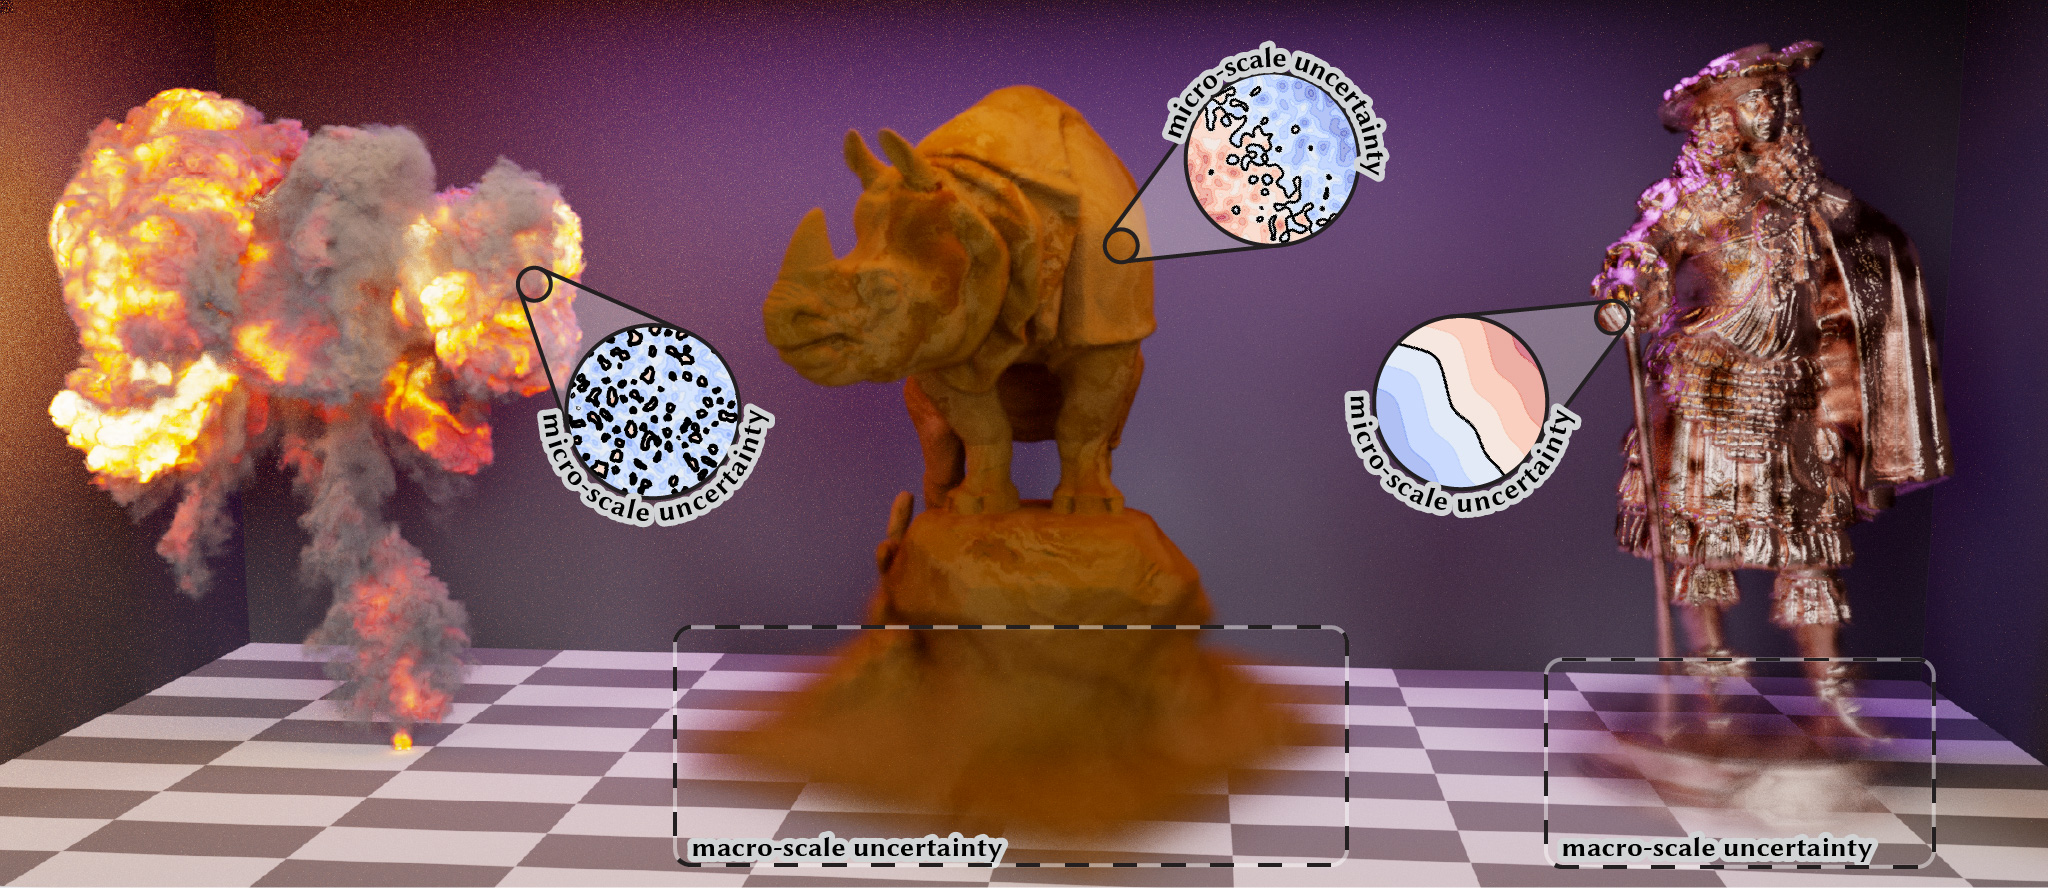
\includegraphics[width=\textwidth]{figures/seyb24from-teaser.jpg}
    \caption{Illustration du continuum de représentations permis par la technique GPIS, allant des surfaces lisses aux milieux participants. Image tirée de \textcite{seyb24from}.}
    \label{fig:seyb24-teaser}
\end{figure}

Seyb et al.~\cite{seyb24from} ont utilisé les GPIS pour définir un modèle contrôlable capable de représenter tous les éléments d'une scène comme un continuum. Cela permet la représentation d'une scène à l'aide d'un modèle de transport lumineux unique. Ce continuum est illustré à la figure~\ref{fig:seyb24-teaser}, où l'on observe que les statues prennent une apparence vaporeuse et volumétrique vers le bas de l'image. C'est cette apparence que nous tenterons de reproduire avec les cheveux.

Pour réaliser cette technique, \textcite{seyb24from} ont développé un algorithme mobilisant le conditionnement et l'échantillonnage de surfaces implicites par processus gaussien, qui s'apparente au \textit{raymarching} volumétrique.

\subsubsection{Algorithme de rendu des GPIS}
\label{sec:algorithme-gpis}

L'algorithme de rendu des GPIS utilise le \textit{raymarching} pour trouver les intersections entre le rayon et les modèles. On cherche à définir une distance $t$ pour laquelle le rayon $\mathbf{x} + t\mathbf{w}$ intersecte la surface, définie par $f(\mathbf{x}_t) = 0$. Pour trouver l'intersection, on génère une réalisation 1D du processus gaussien le long du rayon en faisant l'échantillonnage du processus à plusieurs points avec un écart constant afin de localiser le changement de signe de cette fonction 1D. Pour plus de précision, on interpole entre les échantillons qui causent le changement de signe. Une fois le point d'intersection obtenu, on calcule la normale par la méthode du gradient et, avec le point d'intersection et la normale, on peut évaluer le BSDF exactement comme dans un tracé de rayon standard.

\begin{figure}[H]
    \centering
    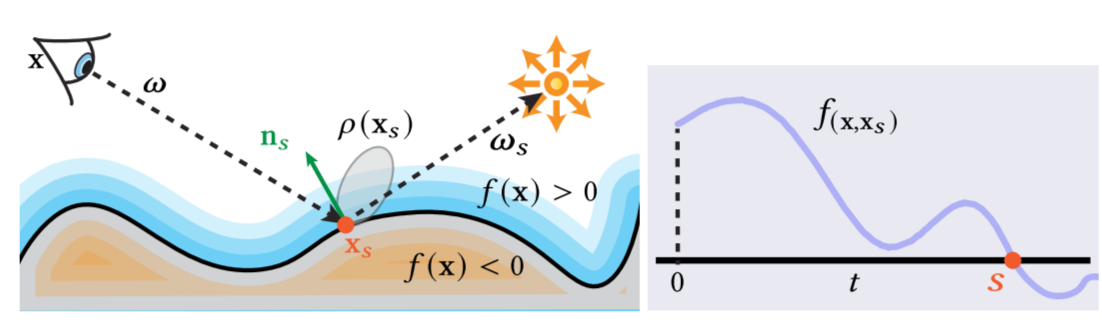
\includegraphics[width=\textwidth]{figures/algorithme-gpis.png}
    \caption{Visualisation de l'échantillonnage le long du rayon pour trouver l'intersection de la surface implicite. Image tirée de \textcite{seyb24from}.}
    \label{fig:algorithme-gpis}
\end{figure}

\subsubsection{Encodage d'un processus gaussien}
\label{sec:encodage-gp}

Ce nouveau type de modèle nécessite un nouveau type d'encodage. Puisque les modèles sont maintenant représentés par un processus gaussien, soit une moyenne et une covariance sous-jacente, il faut être capable de récupérer ces valeurs lors du rendu. Pour ce faire, \textcite{seyb24from} utilisent le format OpenVDB~\cite{museth2013vdb}, qui divise un volume en une grille de cellules 3D (voxels), chacune encodant une valeur. L'utilisation traditionnelle de ce format est d'encoder des propriétés volumétriques telles que la densité de fumée ou des champs de vitesse. En reprenant ce format, les auteurs encodent plutôt la moyenne et la variance du modèle dans chaque voxel ; c'est ainsi que les statues de la figure~\ref{fig:seyb24-teaser} sont représentées. Il est également possible de représenter ces valeurs de façon procédurale, par exemple avec une SDF ou une fonction définie par l'utilisateur comme $ax + b$ pour représenter un plan. Ces trois approches sont implémentées dans Tungsten~\cite{tungsten}, le moteur de rendu développé par Bitterli, l'un des auteurs de l'article.
